%\part{Entwurfsprinzipien} 

%----------------------------------------------------------------------------
\section{Entwurfsprinzipien}
\begin{frame}
\frametitle{Prinzipien f\"ur den objektorientierten Entwurf}
	\begin{itemize}
	  \item Geheimnisprinzip
	  \item Kopplung
	  \item Gesetz von Demeter
	  \item Koh\"asion
	  \item Separation of Concerns
	  \item SOLID
	\end{itemize}
\end{frame}

\begin{frame}[fragile]
	\frametitle{Geheimnisprinzip}
	\begin{itemize}
	  \item Abkapselung von Attributen und innerer Logik von
	  der Au"senwelt
	  \item Methoden werden zu Schnittstellen
	  \item Realisierung durch Modifier:
	  \begin{enumerate}
	    \item public
	    \item private
	    \item protected
	    \item package
	  \end{enumerate}
	\end{itemize}
\end{frame} 

\begin{frame}[fragile]
	\frametitle{Kopplung}
		\begin{itemize}
		  \item Abh\"angigkeit zwischen Klassen
		  \item Kopplung definiert Grad der Abh\"angigkeit
		  \item Zeigt Einfluss von \"Anderungen einer Klassen
		  auf andere Klassen auf
		  \item Ziel: Lose/Geringe Kopplung zwischen Klassen
		  \item L\"asst sich \"uber Metriken messen
		\end{itemize}
\end{frame} 

\begin{frame}[fragile]
	\frametitle{Koh\"asion}
		\begin{itemize}
		  \item Grad des Zusammenhangs aller Verantwortlichkeiten, Daten und
		  Methoden einer Klasse
		  \item Ziel ist eine hohe Koh\"asion innerhalb einer Klasse/Methode\ldots
		  \item L\"asst sich \"uber Metriken messen
		\end{itemize}
\end{frame} 

\begin{frame}[fragile]
	\frametitle{Gesetz von Demeter}
		\begin{itemize}
		  \item Objekte sollen nur mit Objekten in ihrer direkten Umgebung
		  kommunizieren
		  \item Eine Methode sollte nur andere Methoden verwenden
		  	\begin{itemize}
		  	  \item Methoden der eigenen Klasse
		  	  \item Methoden der \"ubergebenen Parameter
		  	  \item Methoden von assoziierten Klassen
		  	  \item Methoden von selbst erzeugten Objekten
		  	\end{itemize}
		\end{itemize}
\end{frame}

\begin{frame}[fragile]
	\frametitle{Gesetz von Demeter}
	\begin{columns}
		\begin{column}{0.5\textwidth}
			Negatives Beispiel:
			\begin{lstlisting}
				class Motor {
					void starten(){}
				}
				
				class Auto {
					private Motor motor;
					
					public Auto() {
						motor = new Motor();
					}
					
					public Motor getMotor(){
						return motor;
					}
				}
				
				class Fahrer(){
					void fahren(){
						Auto a = new Auto();
						Motor m = a.getMotor();
						m.starten();
					}
						
						
					
				}
			\end{lstlisting}
		\end{column}
		\begin{column}{0.5\textwidth}
			Positives Beispiel:
			\begin{lstlisting}
				class Motor {
					void starten(){}
				}
				
				class Auto {
					private Motor motor;
					
					public Auto() {
						motor = new Motor();
					}
					
					public Motor getMotor(){
						return motor;
					}
					
					public void starten(){
						motor.starten();
					}
				}
				
				class Fahrer(){
					void fahren(){
						Auto a = new Auto();
						a.starten();
					}
				}
			\end{lstlisting}
		\end{column}
	\end{columns}
\end{frame}

\begin{frame}[fragile]
	\frametitle{Separation of Concerncs}
	\begin{itemize}
	  \item Aufteilung komplexer Programme/Systeme/Funktionalit\"at nach
	  Verantwortlichkeiten
	  \item Beispielsweise durch Subsysteme oder Schichten
	  \item Vorteile
	  \begin{enumerate}
	    \item Erh\"ohte Qualit\"at durch Nachverfolgbarkeit von 
	    \"Anderung und Wirkung
	    \item Leichtere Austauschbarkeit
	    \item Erh\"ohte Wiederverwendung
	  \end{enumerate}
	\end{itemize}
\end{frame}  

\begin{frame}[fragile]
	\frametitle{SOLID}
		\begin{itemize}
		  \item \begin{emph}S~\end{emph}ingle Responsibility Principle
		  \item \begin{emph}O~\end{emph}pen Closed Principle
		  \item \begin{emph}L~\end{emph}iskov Substitution Principle
		  \item \begin{emph}I~\end{emph}nterface Segregation Principle
		  \item \begin{emph}D~\end{emph}ependency Inversion Principle
		\end{itemize}
\end{frame} 

\begin{frame}[fragile]
	\frametitle{Single Responsibility Principle (SRP)}
	\begin{itemize}
		\item Jede Klasse sollte nur genau EINE fest definierte Aufgabe 
		erf\"ullen
		\item responsibility = 'reason for change'
		\item „Es sollte nie mehr als einen Grund geben eine Klasse zu ändern.“
		\item Einhalten dieses Konzepts impliziert einen sehr hohen Grad der
		Koh\"asion
	\end{itemize}
\end{frame} 

\begin{frame}[fragile]
	\frametitle{Open Closed Principle (OCP)}
	\begin{columns}
		\begin{column}{0.5\textwidth}
			\small
			\begin{itemize}
			  \item Klassen sollen offen f\"ur Erweiterungen
			  aber geschlossen f\"ur Modifikation sein
			  \item Erweiterung: Existierendes Verhalten wird nicht ge\"andert
			  \item Modifikation: \"Anderung von bestehendem Verhalten
			\end{itemize}
		\end{column}
		\begin{column}{0.5\textwidth}
			Negatives Beispiel:
			\begin{lstlisting}
				int melke(Tier t){
					if(t instanceof MilchKuh){
						t.gebeMilch();
					} else if(t instanceof Ziege){
						t.gebeMilch();
					}
				}
			\end{lstlisting}
			Positives Beispiel:
			\begin{lstlisting}
				int melke(Melkbar m){
					m.gebeMilch();
				}
			\end{lstlisting}
		\end{column}
	\end{columns}
\end{frame}  

\begin{frame}[fragile]
	\frametitle{Liskov Substitution Principle (LSP)}
	\begin{columns}
		\begin{column}{0.5\textwidth}
			\small
			\begin{itemize}
			  \item Klassen sollen durch dessen Subklassen ersetzbar sein
			  \item ''Unterklassen sollen nicht mehr erwarten und nicht
			  weniger liefern als ihre Oberklassen''
			\end{itemize}
			
			LSP Versto"s:
			\begin{itemize}
			  \item Kuh spezial = new SpezialKuh();
			  \item spezial.setFarbe(''blau'', ''rot'');
			  \item Annahme: spezial.getFarbe2() = rot
			\end{itemize}
		\end{column}
		\begin{column}{0.5\textwidth}
			\small
			Beispiel f\"ur Versto"s:
			\begin{lstlisting}
				public class Kuh{
					String farbe1;
					String farbe2;
					
					void setFarbe(String f1, String f2){
						farbe1 = f1;
						farbe2 = f2;
					}
					
					String getFarbe1(){
						return farbe1;
					}
					
					String getFarbe2(){
						return farbe2;
					}
				}
				
				public class SpezialKuh extends Kuh{
					void setFarbe(String f1, String f2){
						farbe1 = f1;
						farbe2 = f1;
					}
				}
			\end{lstlisting}
		\end{column}
	\end{columns}
\end{frame} 

\begin{frame}[fragile]
	\frametitle{Interface Segregation Principle (ISP)}
	\begin{columns}
		\begin{column}{0.5\textwidth}
			\small
			\begin{itemize}
			  \item Kopplung erh\"oht durch Verwendung einer
			  globalen Schnittstelle
			  \item \"Anderungen wirken auf beide Nutzer
			\end{itemize}
		\end{column}
		\begin{column}{0.5\textwidth}
			\center
	    	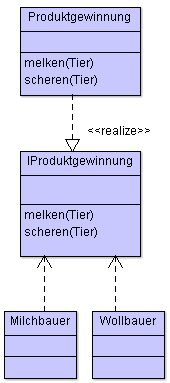
\includegraphics[width=0.5\textwidth,
	    	keepaspectratio=true]{bilder/isp_bad.png}
		\end{column}
	\end{columns}
\end{frame}

\begin{frame}[fragile]
	\frametitle{Interface Segregation Principle (ISP)}
	\begin{columns}
		\begin{column}{0.5\textwidth}
			\small
			\begin{itemize}
			  \item Schnittstellen sollten speziell auf ihre
			  Aufgaben zugeschnitten sein
			  \item ''Clients sollten nicht von Methoden abh\"angen
			  die sie nicht benutzen''
			\end{itemize}
		\end{column}
		\begin{column}{0.5\textwidth}
			\center
	    	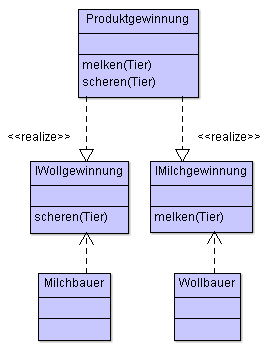
\includegraphics[width=0.6\textwidth,
	    	keepaspectratio=true]{bilder/isp_good.png}
		\end{column}
	\end{columns}
\end{frame}    

\begin{frame}[fragile]
	\frametitle{Dependency Inversion Principle (DIP)}
	\begin{columns}
		\begin{column}{0.5\textwidth}
			\small
			\begin{itemize}
			  \item Module h\"oherer Ebenen sollten nicht von niedrigeren 
			  Modulen abh\"angen
			  \item Abstraktionen h\"angen nicht von Details ab, sondern
			  Details von Abstraktionen
			  \item Abh\"angigkeit immer von konkreten zu abstrakten Programmteilen
			  \item Reduziert Kopplung
			  \item 2 Grundkonzepte:
			  \begin{enumerate}
			    \item Inversion of Control
			    \item Dependency Injection
			  \end{enumerate}
			\end{itemize}
		\end{column}
		\begin{column}{0.5\textwidth}
			\center
	    	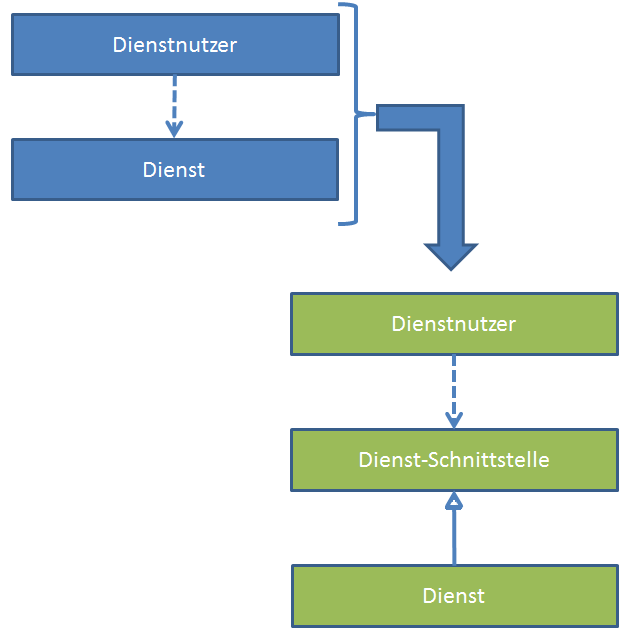
\includegraphics[width=1\textwidth,
	    	keepaspectratio=true]{bilder/dip.png}
		\end{column}
	\end{columns}
\end{frame}

\begin{frame}[fragile]
	\frametitle{Inversion of Control (DIP)}
	\begin{itemize}
	  \item ''Don't call us, we call you''
	  \item Kontrolle der Ausf\"uhrung liegt bei Framework,
	  nicht bei Klassen die es nutzen
	  \item Umsetzung durch Callback-Methoden
	\end{itemize}
\end{frame}   

\begin{frame}[fragile]
	\frametitle{Dependency Injection (DIP)}
	\begin{itemize}
	  \item Problem: Wie kann zur Laufzeit konkrete Implementierung
	  einer Schnittstelle erzeugt werden?
	  \item L\"osung: Dependency Injector\\
	  Er entscheided und ''injiziert'' die ben\"otigte Implementierung
	  der Schnittstelle
	  \item Umsetzung durch Callback-Methoden
	\end{itemize}
	\begin{center}
		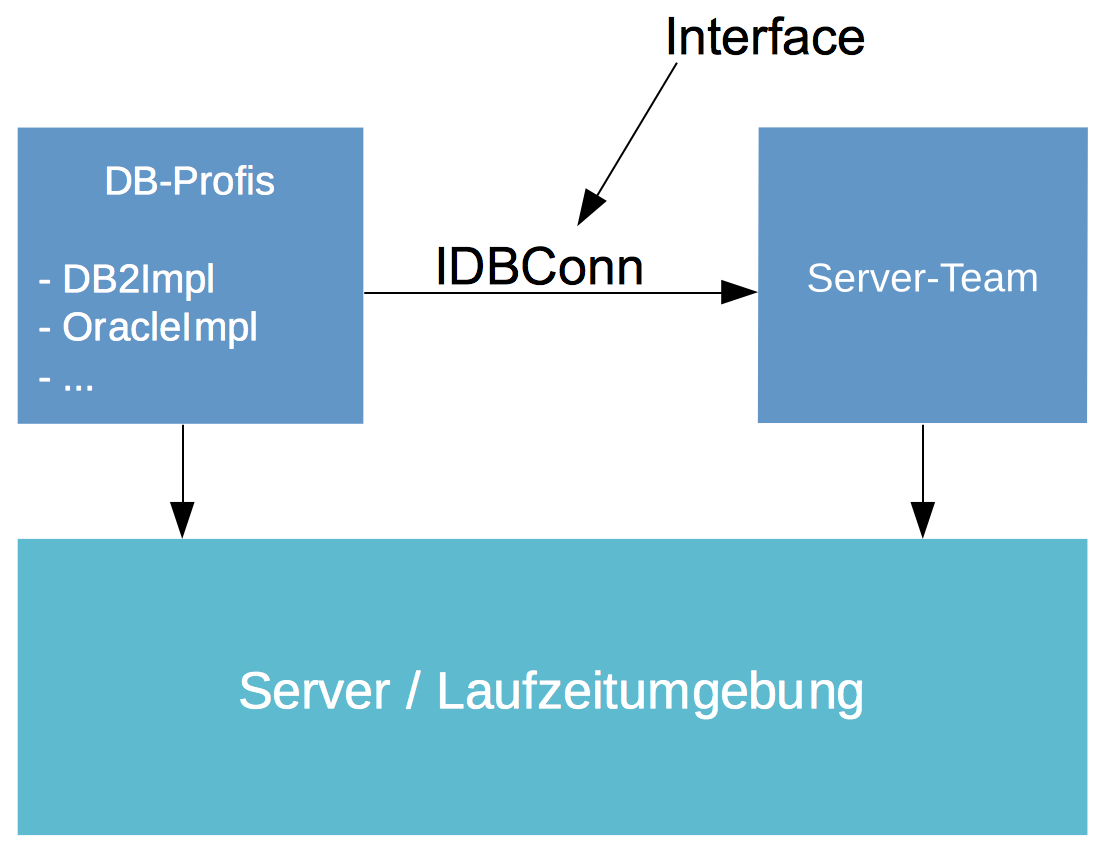
\includegraphics[width=0.6\textwidth,
		keepaspectratio=true]{bilder/dependancy_injection.png}
	\end{center}
\end{frame}

\begin{frame}[fragile]
	\frametitle{Fortgeschrittene OO: Anti-For}
	\begin{center}
		\huge Diskussion!
	\end{center}
\end{frame} 